%\documentclass{beamer}
%
%\usepackage{pgfpages} %This is needed for notes presentation!
%%\setbeameroption{}
%
%\usepackage{enumerate, amsmath, amssymb,amsthm, amstext,color}
%\usepackage[ngerman]{babel}
%\usepackage[utf8]{inputenc}   
%\usepackage{dsfont}
%\usepackage{geometry}
%\usepackage{fancyhdr}
%\usepackage{tikz}
%\usetikzlibrary{plotmarks}
%\usetikzlibrary{arrows, positioning}
%
%\usepackage{float}
%\usepackage{color}
%\usepackage{hyperref}
%% \usepackage{algorithmicx}
%% \usepackage{algpseudocode}
%\usepackage{fancybox}
%\usepackage{float}
%\usepackage{sidecap}
%\usepackage[ngerman]{babel}
%
%
%\newcommand{\lk}{\left}
%\newcommand{\rk}{\right}
%\newcommand{\rel}{\sqsubseteq}
%\newcommand{\rhn}{\mathds{R}^n}
% 
%  \usetheme{Berlin}
%%\usetheme{
%%	AnnArbor | Antibes | Bergen |
%%	Berkeley | Berlin | Boadilla |
%%	boxes | CambridgeUS | Copenhagen |
%%	Darmstadt | default | Dresden |
%%	Frankfurt | Goettingen |Hannover |
%%	Ilmenau | JuanLesPins | Luebeck |
%%	Madrid | Malmoe | Marburg |
%%	Montpellier | PaloAlto | Pittsburgh |
%%	Rochester | Singapore | Szeged |
%%	Warsaw
%%}
%\usecolortheme{beaver}
%% \usecolortheme{
%% 	albatross | beaver | beetle |
%% 	crane | default | dolphin |
%% 	dove | fly | lily | orchid |
%% 	rose |seagull | seahorse |
%% 	sidebartab | structure |
%% 	whale | wolverine
%% }
%
%\useinnertheme{rounded}
%% \useinnertheme{
%% 	circles | default | inmargin |
%% 	rectangles | rounded
%% }
%
%\useoutertheme{infolines}
%% \useoutertheme{
%% 	default | infolines | miniframes |
%% 	shadow | sidebar | smoothbars |
%% 	smoothtree | split | tree
%% }
%
%\usefonttheme{default}
%% \usefonttheme{
%% 	default | professionalfonts | serif |
%% 	structurebold | structureitalicserif |
%% 	structuresmallcapsserif
%% }
%
%% Seitenzahlen
%\setbeamertemplate{footline}[frame number]
%
%\title{Mid-term presentation}
%\author{The Quadrocopters}
%\institute{Technische Universität München}
%\date{\today}
%% \titlegraphic{\pgfimage[width=1cm,height=1cm]{MA_Web}}
%%\logo{\pgfimage[width=1.2cm,height=1.2cm]{MA_Web}}
%
%
%%\AtBeginSection[]{
%%	\frame{
%%	\frametitle{\"Ubersicht}
%%	\tableofcontents[current, currentSection]}
%%
%%}
%
%\setcounter{MaxMatrixCols}{20}
%
%\begin{document}

\definecolor{green}{RGB}{0,190,45}
\definecolor{green2}{RGB}{0,150,45}
\definecolor{red}{RGB}{190,0,0}
\definecolor{blue}{RGB}{0,0,190}

%\begin{frame}
%\maketitle
%\end{frame}
%
%\begin{frame}
%\tableofcontents
%\end{frame}

\section{Realtime Optimization Approach}
\begin{frame}{Setting}

\begin{figure}
\begin{tikzpicture}[scale=1.2]

%Draw bounding box
\draw (-2.75,-1.75) rectangle (3.75,3.25);

%Draw time line
\draw[ thick, ->] (-2.5,0) -- (2,0) node[anchor=west] {time};
\foreach  \t in  {-2, -1, +1}
	\draw[thick]  (\t cm, 1pt)  -- (\t cm, -1pt) node[anchor=north] {\footnotesize $t \t $ };
\draw[thick]  (0cm , 1pt)  -- (0 cm, -1pt) node[anchor=north] {\footnotesize $t$ };

%draw known controls
\draw<2-> (2,1) node[anchor=west] {control};
\draw<2->[->,green] (-2.5, 0.8) -- (-2,0.8) ;
\draw<2->[->,green] (-2, 1.2) -- (-1,1.2) ;
\draw<2->[->,green] (-1, 0.9) -- (0,0.9) ;
\draw<4->[->,red,thick] (0, 1.1) -- (1,1.1) ;

%Draw actual time
\draw[dashed] (-.65,3) -- (-.65,-1) node[anchor=north] {$t_{act}$};

%Draw exact states
\draw<2-> (2,2) node[anchor=west] {state};
\draw<2->[green, fill=green] (-2, 2.2) circle (1pt) node[anchor=north]{\footnotesize $x_{t-2}$};
\draw<2->[green, fill=green] (-1, 1.9) circle (1pt) node[anchor=north]{\footnotesize $x_{t-1}$};
\draw<3->[red, fill=red] (0,2.1) circle (1pt) node[anchor=north]{\footnotesize $x_{t}$};
\end{tikzpicture}
\end{figure}
\end{frame}

\begin{frame}{Discrete Problem}
\begin{block}{}
\small{
\begin{align*}
  \min_{s, q} \sum_{i=t}^{N-1} J_{i}(s_{i},q_{i}) \ \  
  s.t. \ \left\lbrace \begin{array}{rl}
  x_{t} - s_{t} = 0 & \\
  h_i (s_i ,q_i ) - s_{i+1} = 0 & \forall i = t, ... , N-1 \\
  p_{A_i}(s_i, q_i) = 0 & \end{array} \right. 
\end{align*}}
\end{block}
\vspace{1ex}
\begin{tabular}{l l}
  $J_i(s_i, q_i)$ &  discretized goal function 
  \vspace{1ex} \\
$x_t - s_t = 0$ & expected state $=$ real state
  \vspace{1ex} \\
$h_i (s_i ,q_i )$ & solution of the ODE at time $i$ 
  \vspace{1ex} \\
$p_{A_i}(s_i, q_i)$ & activ inequality constraints\\
\end{tabular}
\end{frame}

\begin{frame}{The Lagrangian}
\begin{block}{ }
\begin{align*}
\begin{array}{r l}
  L^{t}(y) = &  \sum\limits_{i=t}^{N-1} J_{i}(s_{i},q_{i})
  + \lambda_{t}^{T}(x_{t} - s_{t}) \\
  & + \sum\limits_{i=t}^{N-1} \lambda_{i+1}^{T} (h_i (s_i ,q_i ) - s_{i+1}) \\
  & + \sum\limits_{i=t}^{N-1} \mu_{i}^{T} p_{A_i}(s_i,q_i)
  \end{array}
\end{align*}
\vspace{.1ex}
\end{block}
$$ y := (\lambda,s,q,\mu) $$
\vspace{1ex}
Search for optimal $y^*$ : \\
\[ \Rightarrow \nabla_{y} L^{t}(y^*)  = 0 \]

\end{frame}

\begin{frame}{The SQP Method}
How to find $y^*$?
\begin{block}{ }
\begin{gather*}
y_{k+1} = y_{k} + \alpha_{k} \Delta y_{k}  \\ 
\min_{\Delta y_k}  \frac{1}{2} \Delta y_k^T A_k \Delta y_k + \nabla_{y_k} J(y_k)^T \Delta y_k
\end{gather*} \vspace{.1ex}
\end{block}
\onslide<2->
\vspace{1ex}
Special case: \\
\vspace{1ex}
\begin{tabular}{l l}
$ A_{k} = H(y_k)$ & approximated Hessian $\nabla^{2}_{y_k} L(y_k)$ \vspace{1ex} \\
$\alpha_k = 1$ & 
\end{tabular}
\end{frame}

\begin{frame}{Newton-Methode}
Find $\Delta y_k$ with:
\begin{block}{}
\begin{gather*}
\nabla_{y_k} L(y_{k}) + H(y_{k}) \Delta y_{k} = 0
\end{gather*} \vspace{.1ex}
\end{block}
\onslide<2->
1 iteration per timestep:
\begin{block}{ }
\begin{gather*}
y_{t+1} = y_1 = y_0 + \Delta y_0 \\
\end{gather*}
\end{block}
\end{frame}

\begin{frame}{Riccati Recursion}

Solves linear system fast
\begin{figure}
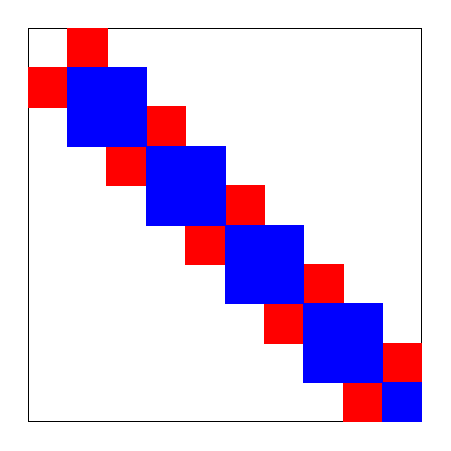
\begin{tikzpicture}
%Draw bounding box
\draw[black] (-1.5,-4.5) rectangle (3.5,0.5);

\draw[blue,fill=blue] (-1,0.5) rectangle (-0.5, 0);
\draw[blue,fill=blue] (-1.5,0) rectangle (-1, -0.5);
\draw[blue,fill=blue] (-0.5,-0.5) rectangle (0.5, -1.5);
\draw[blue,fill=blue] (0.5, -1.5) rectangle (1.5, -2.5);
\draw[blue,fill=blue] (1.5, -2.5) rectangle (2.5, -3.5);
\draw[blue,fill=blue] (2.5, -3.5) rectangle (3.5, -4.5);

\draw<2->[red,fill=red] (-1,0.5) rectangle (-0.5, 0);
\draw<2->[red,fill=red] (-1.5,0) rectangle (-1, -0.5);
\draw<2->[red,fill=red] (-0.5,-0.5) rectangle (0.5, -1.5);
\draw<2->[red,fill=red] (0.5, -1.5) rectangle (1.5, -2.5);
\draw<2->[red,fill=red] (1.5, -2.5) rectangle (2.5, -3.5);
\draw<2->[red,fill=red] (2.5, -3.5) rectangle (3.5, -4.5);

\draw[blue,fill=blue] (-1,0) rectangle (0, -1);
\draw[blue,fill=blue] (0,-1) rectangle (1, -2);
\draw[blue,fill=blue] (1,-2) rectangle (2, -3);
\draw[blue,fill=blue] (2,-3) rectangle (3, -4);
\draw[blue,fill=blue] (3,-4) rectangle (3.5, -4.5);

\end{tikzpicture} 
\end{figure}

%\textit{\begin{align*} 
%  \scriptstyle{H^{t}(y^{t})} =
%  \tiny{
%	\begin{pmatrix}
%		& -E  &     &     &     &     &     &     &     &     &     \\ \\
%-E  & Q_t^{H} & M_t^{H} & A_t^{T} &  &    &     &     &     &     &     \\ \\
%    & (M_t^{T})^{H} & R_t^{H} & B_t^{T} &   &    &    &    &    &   &     \\ \\
%    & A_t & B_t &     & -E  &     &     &     &     &     &     \\ \\
%    &  &  & -E  & Q_{t+1}^{H} & M_{t+1}^{H} & A_{t+1}^{T} &  &  &  &  \\ \\
%    &  &  &     & (M_{t+1}^{T})^{H} & R_{t+1}^{H} & B_{t+1}^{T} &  &  &  &  \\ \\
%    &  &  &     & A_{t+1} & B_{t+1} &    &    &     &     &     \\ \\
%    &  &  &     &    &    &   & \ddots &     &     &     \\ \\
%    &  &  &   &  &  & \ddots & Q_{N-1}^{H} & M_{N-1}^{H} & A_{N-1}^{T} &  \\ \\
%    &  &  &   &  &  &    & (M_{N-1}^{T})^{H} & R_{N-1}^{H} & B_{N-1}^{T} &  \\ \\
%    &  &  &   &  &  &    & A_{N-1}     & B_{N-1} &    & -E \\ \\
%    &  &  &     &    &    &     &      &     & -E &  Q_N^{H} 
%\end{pmatrix}
%}
%  \end{align*}}

\end{frame}

\begin{frame}{Summary}
What happens in interval $ [ t-1 , t ] $ ?
\begin{figure}
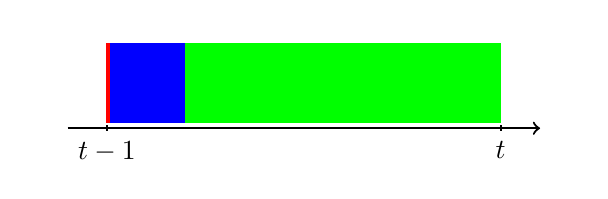
\begin{tikzpicture}
%Draw bounding box
\draw[white] (-1,-.5) rectangle (6,1.2);

%Draw time line
\draw[ thick, ->] (-.5,-2pt) -- (5.5,-2pt);

\draw[thick]  (5 cm, -1pt)  -- (5 cm, -3pt) node[anchor=north] {$t$ };
\draw[thick]  (0cm , -1pt)  -- (0 cm, -3pt) node[anchor=north] {$t-1$ };

%Solve for control in t_k-1
\draw<2->[red,fill=red] (0,0) rectangle (0.05, 1);
% Calculcate start value for t_k
\draw<3->[blue,fill=blue] (0.05,0) rectangle (1, 1);
%Prepare for t_k
\draw<4->[green, fill=green] (1,0) rectangle (5,1);
\end{tikzpicture}
\end{figure}

\begin{enumerate}
\item<2-> {\color{red} calculate control $u_{t-1}$ (Riccati Part II)}
\item<3-> {\color{blue} calculate $y$ (Riccati Part II)}
\item<4-> {\color{green2} prepare $u_t$ (Newton \& Riccati Part I)} 
\end{enumerate}
\end{frame}

\begin{frame}{Finite Horizon}

%\begin{itemize}
%\item $N=t_{end} \rightarrow $ problem gets smaller every time 
%\item $N=t+n \rightarrow $ problem size is constant
%\item .
%\item .
%\item .
%\end{itemize}
\begin{block}{}
\small{
\begin{align*}
  \min_{s, q} \sum_{i=t}^{N-1} J_{i}(s_{i},q_{i}) \ \  
  s.t. \ \left\lbrace \begin{array}{rl}
  x_{t} - s_{t} = 0 & \\
  h_i (s_i ,q_i ) - s_{i+1} = 0 & \forall i = t, ... , N-1 \\
  p_{A_i}(s_i, q_i) = 0 & \end{array} \right. 
\end{align*}}
\end{block}
\vspace{1ex}
How to choose $N$? \\
\vspace{1ex}
\begin{tabular}{l l}
$N=t_{end} $ &$ \rightarrow $ problem size decreasing \\ \vspace{1ex}
\onslide<2->
$N=t+n $ & $\rightarrow $ problem size constant \\
\end{tabular}

\end{frame}
%\end{document}